%!TEX root = /Users/manunavjeevan/Documents/GitHub/mnavjeev.github.io/files/Moment Inequality Methods/Annotated Literature Review/inequalityLitReview.tex

\newpage
\section{A Geometric Approach to Inference in Set-Identified Entry Games; \textit{\small Christian Bontemps, Rohit Kumar (JoE, 2020)}}\label{sec:BK-2020}

\citet{BK-2020} is set to appear in Journal of Econometrics in 2020. They consider inference procedures for entry games with complete information. Complete the model with the unknown selection mechanism and characterize geometrically the set of predicted choice probabilities. A 2019 version of the paper can be found 
\href{https://www.cemmap.ac.uk/uploads/Bontemps-Kumar-JofEc-december2019.pdf}{here}.

\subsection{Introduction}

Paper provides an estimation procedure for empirical models of entry and market structure. Entry games are popular in the empirical Industrial Organization literatures because they allow researchers to study the nature of firms' profits and the nature of competition between firms from data that are generally easy to collect. Popularized by the seminal works of Bresnahan and Reiss (1991a). 

Econometrics analysis of entry games is complicated by the presence of multiple equilibria, a problem that affects the standard estimation strategy.  Without additional assumptions, the model is incomplete. 

This paper completes the model with the selection mechanism $\eta(\cdot)$ and characterizes the set of predicted choice probabilities generated by the variation of $\eta(\cdot)$ in the space of admissible selection mechanisms. First contributions is to characterize more deeply the geometric structure of this set. 

Set ends up being a convex polytope with many facets (because of focus on pure strategy equilibrium). This paper derived a closed form expression for the support function of this polytope, the extreme points (or \emph{vertices}) of which can also be calculated as a function of the primitives of the model. Vertices are characterized by an order of outcome selection in the regions of multiple equilibria. Each vertex is also geometrically defined by the intersection of some supporting hyperplanes. Able to define the cone of outer normal vectors of these hyperplanes, and, thereby, the inequalities that are binding in this point.

Testing whether a parameter belongs to the identified set is equivalent to testing whether the true choice probability vector belongs to this convex set. However, when the number of players increases, the number of facets of the polytope increases exponentially, and, therefore, the smallest number of inequalities necessary to have a sharp characterization of the the identified set - from 16 in a game with 3 players to more than 1 million in a game with 6 players.

\subsection{Entry Game with \emph{N} players}

Formalize the entry game considered with $N$ firms. First consider a model without explanatory variables.

\subsubsection{Setup and Notations}

\paragraph{Model}
Let $N$ denote the number of firms that can enter any market. Following Berry (1992), introduce a model of market structure where the profit function $\pi_{im}$ of firm $i$ in a market $m$ is assumed to be independent of the identity of the firm's competitors. All firms decide simultaneously whether to enter the market (action \(a_{im} = 1\), doing so if their profit is positive. If $\pi_{im} = 0$, firms do not enter the market (take action \(a_{im}= 0\)). The profit function is assumed, without loss of generality, to be linear in the explanatory variables\footnote{[FOOTNOTE FROM TEXT] Any separable parametric form $\pi_{im} = f_i(\sum_{j\neq i} a_{jm}l\alpha) + \eps_{im}$ can be considered as long as the function $f_i(\cdot;\theta)$ is strictly decreasing in its first argument.}
\begin{equation}
	\label{eq:BK-1}
	\begin{split}
    	\pi_{im} &= \beta_i + \alpha_i \left(\sum_{j\neq i}a_{jm}\right) + \eps_{im} \\
    	a_{im} &= \ind\{\pi_{im} > 0\}
	\end{split}
\end{equation}


Following the literature, assume that $\alpha_i < 0$, i.e, the presence of more competitors decreases a firm's profit. Unobserved components $\eps_{im}, i = 1,\dots, N$ are drawn from a known distribution (up to some parameter vector $\gamma$). Econometrician does not observe their values but firms do.

For identification, we first need a scale normalization, and thus, assume that the variance of each shock $\eps_{im}$ is equal to 1. Denote the distribution of $\eps_m = (\eps_{1m},\dots, \eps_{Nm})^T$ and assume that the distribution is continuous with full support. Use notation $\theta$ for all the parameters in the model, and omit the subscript $m$ for notational convenience. Assume $\theta \in \Theta \subseteq \SR^l$. 

\paragraph{Multiplicity of Pure Strategy eqm.}

For a given market, an outcome $y$ is the vector of actions (in $\{0,1\}^N$) taken by the firms. There are $2^N$ possible outcomes. Denote by $\calY$ this set of possible outcomes. $\calY_K$ denotes the subset of outcomes with $K$ active firms in equilibrium, i.e any firms playing action 1. There is 1 outcome with 0 active firms, $N$ outcomes  with 1 active firm, $d_k = \binom{N}{K}$ with $K$ active firms, etc. 

Globally, order the outcomes in $\calY$ first by their number of active firms, then according to the predefined order within each $\calY_K$:
\[\calY = \left\{\underbrace{y_1^{(0)}\vphantom{,\dots,y_{d_K}^{(N)}}}_{\calY_0}, \underbrace{y_1^{(1)}, \dots, y_{d_1}^{(1)}}_{\calY_1}, \dots, \underbrace{y_1^{(K)},\dots,y_{d_K}^{(K)}}_{\calY_K},\dots, \underbrace{\vphantom{,\dots,y_{d_K}^{(N)}}y_1^{(N)}}_{\calY_N} \right\}\]

Well known that the model has multiple equilibria, regions of realizations of $\eps$ in which one cannot uniquely predict each firms' action. Consequently, no one-to-one mapping between the collection of possible outcomes and the regions of $\eps$ given any parameter value $\theta$. Consequently no one-to-one mapping between the collection of possible outcomes and the regions of $\eps$ given any parameter value $\theta$. 

Missing from the model is the selection of a given equilibrium in the regions of multiple equilibria. Define this selection mechanism $\eta(\cdot)$ as in Definition \ref{def:GH-2} of \citet{GH-2011}.

\begin{definition}[Equilibrium Selection Mechanism]
	\label{def:BK-1}
	An equilibrium selection mechanism is a conditional probability $\eta(\cdot | \eps; \theta)$ such that the selected value of the outcome variable is actually an equilibrium predicted by the game. That is $\supp(\eta(\cdot | \eps;\theta)) \subseteq G(\eps |\theta) $
\end{definition}

Denote by $\calE$ the set of selection mechanisms and by \(P(\theta,\eta)\) the predicted choice probability vector when the parameter of the model is is \(\theta\) and selection mechanism is $\eta(\cdot)$. Partition this vector according to the partition of $\calY$ as 
\begin{equation}
	\label{eq:BK-2}
	P(\theta,\eta) = \left(\underbrace{\vphantom{,\dots P_{d_k}^{(K)}(\theta,\eta)}P_1^{(0)}(\theta,\eta)}_{P^{(0)}(\theta,\eta)},\dots, \underbrace{P_1^{(K)}(\theta,\eta),\dots, P_{d_K}^{(K)}(\theta,\eta)}_{P^{(K)}(\theta,\eta)},\dots\underbrace{\vphantom{,\dots P_{d_k}^{(K)}}P_1^{(N)}(\theta,\eta)}_{P^{(N)}(\theta,\eta)}\right)^T
\end{equation}

One solution to the multiple equilibria problem consists of making assumption on this selection mechanism like in Reiss (1996) or Cleeren (2010). The vector of predicted choice probabilities is a point in $[0,1]^{2^N}$ and standard inference techniques may be used. Of course, any restrictions are ad hoc and may lead to misspecification. 

Another solution, following the literature on set-identification, consists of characterizing all the possible choice probabilities predicted by the model. The vector of predicted choice probabilities, instead of being an unrestricted point, belongs to a convex set that is characterized. Different sets of values $(\theta, \eta)$ may generate the same point $P(\theta,\eta)$. Goal is to characterize which ones generate the true (read: observed) choice probability vector. 

\subsubsection{Choice Probabilities to Identified Set}

Want to characterize the set of predicted choice probabilities. To do so, need to understand the multiplicity structure and characterize it. Then derive a parameterization of the set. 

\paragraph{Regions of Multiple Equilibria}

Specification ensures that multiple equilibria only involve outcomes with the same number of active firms, i.e within $\calY_K$. Therefore, focus on subsets of outcomes $S\subseteq \calY_K$ to characterize the multiple equilibria regions. Say that a subset $S\subseteq \calY_k$ is \textbf{in multiplicity} if the prediction of the game is all outcomes in $S$ and no outcome outside $S$ for $\eps$ in a non empty set $\calR_S^{(K)}(\theta)$.\footnote{In the Galichon Henry (2011) notation, this means that \(S = G(\eps|\theta)\) for some \(\eps \in \calU\). Then $\calR_S^{(K)}(\theta) = \{\eps \in \calU : G(\eps|\theta) = S\}$}
$\calR_S^{(K)}$ is called a multiple equilibria region. Denote by $S^{(K)}$ the collection of subsets $S$ of $\calY_K$ in multiplicity\footnote{The maximum number of such subsets is equal to $2^{d_K} - d_k - 1$}.
\[S^{(K)} = \left\{S\subset \calY_K: |S|\geq 2\text{ and $S$ is in multiplicity}\right\}\]
Note that not all subsets of cardinality greater than two are elements of $S^{(K)}$. For example, when $N = 4$, $K = 2$, $S_1 = \{(1,1,0,0)^T,(0,0,1,1)^T\}$ is not in multiplicity whereas the subset $S_2 = \{(1,1,0,0)^T,(1,0,1,0)^T\}$ is\footnote{This just means that, there exists a value of $(\theta,\eps)\in \Theta \times \SR^{N}$ such that both outcomes in $S_2$ are simultaneously equilibria of the game. That is, given $\theta$ and $\eps$, both $(1,1,0,0)^T$ and $(1,0,1,0)^T$ are equilibria. However, there is no value of $(\theta,\eps)$ such that both $(1,1,0,0)^T$ and $(0,0,1,1)^T$ are both simultaneously equilibrium outcomes.}.

Now present necessary and sufficient condition for $S$ to be in multiplicity. 
\begin{align*}
	N_0(S) &= \{\text{Set of indices of firms that always play action 0 across $S$}\} \\
	N_1(S) &= \{\text{Set of indices of firms that always play action 1 across $S$}\} 
\end{align*}
Further define $n_0(S) = |N_0(S)|$ and $n_1(S) = |N_1(S)|$, the cardinalities of the sets above. For now, suppress the dependence on $S$. With $N_0$ and $N_1$ fixed, there are $\binom{N - n_0 - n_1}{K - n_1}$ possible outcomes in $\calY_K$ corresponding to the remaining choice of the $K-n_1$ which play action $a_{im} = 1$ among the $N- n_0 - n_1$ remaining ones. $S$ should contain all these possibilities to be in multiple equilibria. 
\begin{prop}
	\label{prop:BK-1}
	A set $S\subset \calY_K$ is in multiplicity if and only if \(|S| = \binom{N- n_0 - n_1}{K - n_1}\)
\end{prop}
For the particular examples above, $S_1$ is not in multiplicity because $n_0 = n_1 = 0$ and, consequently, the subset should contain $\binom{4}{2} = 6$ outcomes with two active firms to be in multiplicity. $S_2$ is in multiplicity because $n_0 = n_1 = 1$ and it collects all possible outcomes, \(\binom{4-1-1}{2-1}=1\). Proof of proposition 1 also characterizes the region \(\calR_S^{(K)}(\theta)\).  Proposition \ref{prop:BK-1} can be used to count the number of multiple equilibria regions:
\begin{prop}
	\label{prop:BK-2}
	The cardinality of $S^{(K)}$, i.e, the number of multiple equilibria regions predicting $K$ active firms, for $1\leq K \leq N-1$ is equal to 
	\[|S^{(K)}| = \sum_{n_1 = 0}^{K-1} \sum_{n_0 = 0}^{N-K-1}\binom{N}{n_1}\binom{N-n_1}{n_0}\footnote{We can think of this as, for a given $K$ firms that are active in the quilibrium, choose $n_1$ to ``always'' be in and $n_0$ to ``always'' be out. So long as $n_0 + n_1 < N$ and $n_1 < K$, there is garunteed to be a region of mulitple equilibria corresponding to this by Proposition \ref{prop:BK-1}.}\]
\end{prop}
With $K=1$, the number of regions of multiple equilibria is $\sum_{n=0}^{N-2} \binom{N}{n}$, all possible combinations of more than two outcomes. However, Table \ref{table:BK-1} shows that the number of regions for the various values of $N$ and $K$ is generally far less than all the possible combinations. So the parameterization of the set of predicted choice probabilities is of a much lower dimension than one would have expected.
\begin{table}[htb!]
	\centering
	\begin{tabular}[c]{|lllll|}
		\hline\hline
		$N$ & $K$ & $d_k$ & $|S^{(K)}|$ & $2^{d_k} - d_k - 1$\\
		\hline
		3 & 1 & 3 & 4 & 4 \\ 
		  & 2 & 3 & 4 & 4 \\
		\hline 
		4 & 1 & 3 & 11 & 11 \\ 
		& 2 & 6 & 21 & 59 \\ 
		& 3 & 4 & 11 & 11 \\ 
		\hline 
		5 & 1 & 5 & 26 & 26 \\
		& 2 & 10 & 71 & 1018 \\
		& 3 & 10 & 71 & 1018 \\
		& 4 & 5 & 26 & 26 \\
		\hline 
		6 & 1 & 6 & 57 & 57 \\
		& 2 & 15 & 198 & 32761\\
		& 3 & 20 & 283 & 1048569 \\
		& 4 & 14 & 198 & 32761 \\ 
		& 5 & 6 & 57  & 57\\
		\hline\hline
	\end{tabular}
	\caption{Counting the number of multiple equilibria regions [Lifted from paper]}
	\label{table:BK-1}
\end{table}

\paragraph{The set of predicted choice probabilities} Also define the subset of $S^{(K)}$ that contains one specific outcome $y_j^\PK$ as 
\[S_j^\PK = \left\{S\in S^\PK : y_j^\PK \in S\right\}\]
Following \citet{BT-2007} and \citet{GH-2011}, can calculate the probability of observing outcome $y_j^\PK$. This probability depends on the parameter vector $\theta$ and the selection mechanism $\eta$. Specifically, letting $U_j^\PK(\theta)$ be the region in the support of $\eps$ which uniquely predicts the outcome $y_j^\PK$:
\begin{equation}
	\label{eq:BK-3}
	P_j^\PK(\theta,\eta) = \int_{U_j^\PK(\theta)} dF(\eps;\theta) + \sum_{S\in S_j^\PK} \int_{R_S^\PK(\theta)} \eta\left(y_j^\PK|\eps;\theta\right) dF(\eps;\theta)
\end{equation}
Denote by 
\[\Delta_j^\PK(\theta) :=\int_{U_j^\PK(\theta)} dF(\eps;\theta)\andbox \Delta_S^\PK(\theta) := \int_{R_S^\PK(\theta)} dF(\eps;\theta)\]
Let $A(\theta)$ be the set of $P(\theta;\eta)$ generated by the variation of $\eta$ in $\calE$\footnote{Recall \(\calE\) is the set of all valid equilibrium selection mechanisms.} and let $B_K^\theta$ be the set of $P^\PK(\theta, \eta)$ generated by the variation of $\eta$ in $\calE$, for $K = 0,\dots,N$. Formally
\[A(\theta):= \left\{P\in\SR^{2^N}: \exists \eta \in \calE, P = P(\theta,\eta)\right\} \andbox B_K(\theta) := \left\{P^\PK\in \SR^{d_K}: \exists \eta \in \calE, P^\PK = P^\PK(\theta, \eta) \right\}\]
Equation \ref{eq:BK-3} can then be viewed as a parameterization of the sets $A(\theta)$ and $B_K(\theta)$ where the ``parameters'' are the regions $\calR_S^\PK(\theta)$\footnote{This means that elements of the sets $A(\theta)$, $B_K(\theta)$ are characterized/fully determined by their corresponding regions $\calR$.}.

\paragraph{A characterization of the identified set} 

Let $P_0 = P(\theta_0,\eta_0)$ be the true choice probabilities generated by the ``true'' unknown parameter and selection mechanism. The identified set $\Theta_I$ is defined as the collection of points $\theta$ such that $P_0$ can be rationalized with a selection mechanism 
\begin{equation}
	\label{eq:BK-4}
	\Theta_I := \left\{\theta\in \Theta: \exists \eta\in\calE, P_0 = P(\theta,\eta) \right\}
\end{equation}
The following is easily verified and intuitive
\begin{equation}
	\label{eq:BK-5}
	\theta\in\Theta_I \iff P_0 \in A(\theta)
\end{equation}
So, can study $\Theta_I$ by studying the structure of $A(\theta)$. The following result holds:
\begin{prop}
	\label{prop:BK-3}
	\(A(\theta)\) is a convex subset of $\SR^{2^N}$, each $B_K(\theta)$ is a convex subset of $\SR^{d_K}$, and 
	\[A(\theta) = B_0(\theta) \times B_1(\theta)\times \dots \times B_N(\theta)\]
\end{prop}
The convexity of $A(\theta)$ is a general feature of an entry game and does not depend on this specification. The specific structure, the direct product nature, comes from the specification in Equation (\ref{eq:BK-1}). Structure simplifies some of the results to follow. 

Also, $B_K(\theta)$ is a point only when the number of active firms in equilibrium is $0$ or $N$, because there is no region of multiple equilibria involving these specific outcomes. Note that each $B_K(\theta)$ is strictly included in the cube, $\cube_K$, defined by 
\begin{equation}
	\label{eq:BK-6}
	\Delta_j^\PK(\theta) \leq P_j^\PK \leq \Delta_j^\PK(\theta) + \sum_{S\in S_j^\PK} \Delta_S^\PK(\theta), \forall j \in \{1,\dots, d_K\}
\end{equation}
This follows simply from the breakdown of $P_j^\PK$ in equation (\ref{eq:BK-3}), the following definitions of $\Delta_j^\PK$ and $\Delta_S^\PK(\theta)$, and that $0 \leq \eta(\cdot) \leq 1$.

$\Theta_I$, the identified set, is not convex, but it can be characterized by verifying that a point $P_0$ belongs to a convex set $A(\theta)$. Using Proposition \ref{prop:BK-3}, can decompose this condition to
\[P_0\in A(\theta)\iff \forall K \in \{0,1,\dots, N\}, P_0^\PK \in B_K(\theta)\]
\subsubsection{The Support Function and a First Selection of Moment Inequalities}

Following the convex literature, introduce the support function of each convex set $B_K(\theta)$. Tool has, in particular, been used in the set-identified literature, by Beresteanu and Molinari (2008) and Bontemps et al. (2012). Helps in generating the set of inequalities satisfied by $P_0$. First go over what a support function of a convex set is, and how it generates the inequalities that are the basis of inference procedure. The \emph{support function} of a convex set $A\subset \SR^d$ is defined as 
\[\delta^*(q;A)= \sup_{x\in A} q^T x\]
for all directions $q \in \SR^d$. This is depicted visually in Figure \ref{fig:BK-Fig1}, below. Generally, the domain of $\delta(\cdot)$ is restricted to $\mathbb{S}^{n-1}$
\begin{figure}[htb!]
	\centering
	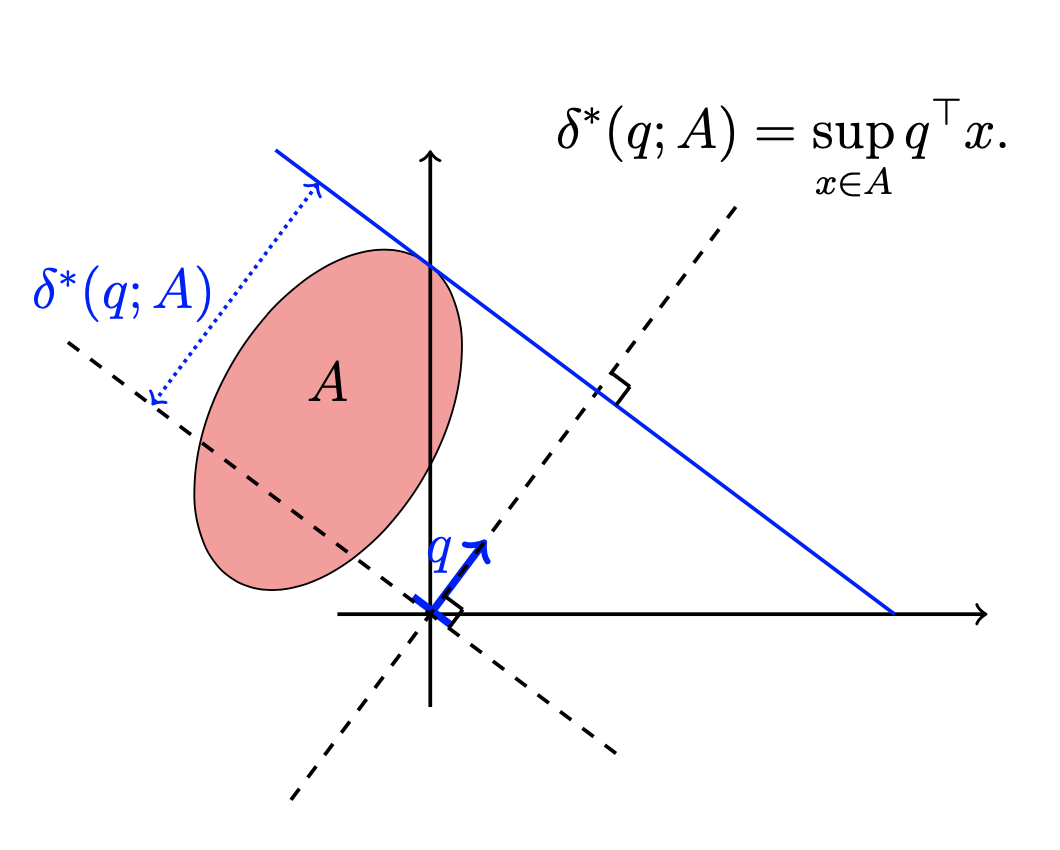
\includegraphics[width=0.50\textwidth]{figures/BK-Fig1.png}
	\caption{The support function [Lifted from \citet{BK-2020}]}
	\label{fig:BK-Fig1}
\end{figure}
The support function of a convex set in a given direction locates the supporting hyperplane in this direction. For each direction $q$, it defines an inequality that is satisfied by any point of the convex set. The support function implicitly gathers all the inequalities that define the convex set into a single function. If the set is smooth, there is a continuum of such inequalities. If it is a polytope, there are only a finite number of (linear) inequalities needed to characterize the set. \citet{KS-2014} show that, when the set is convex, using the support function leads to an efficient estimator of the convex identified set.

Following Rockafeller (1970) and Proposition \ref{prop:BK-3}, the identified set is characterized by the following inequalities.
\begin{equation}
	\label{eq:BK-7}
	\begin{split}
	 	\theta \in \Theta_I &\iff P_0 \in A(\theta) \\ 
	 	&\iff \forall q\in \SR^{2^N}, q^T P_0 \leq \delta^*(a;A(\theta)) \\
	 	&\iff \forall K, P_0^\PK \in B_K(\theta) \\
	 	&\iff \forall K, \forall q_K \in \SR^{d_K}, q_K^T P_0^\PK \leq \delta^*(q_K;B_K(\theta))
	 \end{split} 	
\end{equation} 
Breaking this down. $P_0$ is the observed ``true'' vector of outcome probabilities. \(A(\theta) \subset \SR^{2^N}\) is the set of probabilities that can be rationalized by an equilibrium selection mechanism in the model with parameter vector $\theta$. $P_0^\PK \in \SR^{d_K}$ is the sub-vector of probabilities for outcomes with $K$ active firms, where $d_K = \binom{N}{K}$, the number of possible outcomes with $K$ active firms. $B_K(\theta) \subset \SR^{d_K}$ is the set of sub-vectors of observed probabilities for outcomes with $K$ active firms that can be rationalized by an equilibrium selection mechanism in a model generated by parameter vector $\theta$.

Now turn to the calculation of the support function of $B_K(\theta)$ for any $K$. Make the following notations:
\begin{enumerate}
	\item  Let $q_K \in \SR^{d_K}$ be a given direction. Assume the following order among the coordinates of $q_K$: $q_{i_1,K} \geq q_{i_2,K} \geq \dots, \geq q_{i_{d_K},K}$. 
	\item Partition $S^\PK$, the collection of subsets of outcomes with $K$ active firms in multiplicity, as follows:  
	\begin{enumerate}
		\item Denote $\calO^\PK_{i_1} = S_{i_1}^\PK$\footnote{Remember $S_j^\PK = \{S \in S^\PK: y_j \in S\}$}, the elements of $S^\PK$ which contain the outcome $y_{i_1}^\PK$\footnote{$y_{i_1}^\PK$ being the outcome with $K$ active firms that has the highest probability assigned to it by $q_K \in \SR^{d_K}$}.
		\item Denote by $\calO^\PK_{i_2} \subset S_{i_2}^\PK$ the subset of elements of $S_{i_2}^\PK$ that are not in $\calO_{i_1}^\PK$, i.e $\calO_{i_2}^\PK = S_{i_2}^\PK \setminus S_{i_1}^\PK$.
		\item Continue on in this fashion for each $i_j, j \in 3, \dots, d_K$ defining 
		\[\calO_{i_j}^\PK = S_{i_j}^\PK \setminus \bigcup_{k < j} S_{i_k}^\PK\]
	\end{enumerate}
\end{enumerate}
Note that the construction of the outcomes $\calO_j^\PK$ is lined to the order of the components of $q_k$. Now provide a closed form expression for the support function in this direction (Prop \ref{prop:BK-4}, below).
\begin{prop}
	\label{prop:BK-4}
	Let $q_k\in\SR^{d_K}$ and assume $q_{i_1,K}\geq q_{i_2,K}\geq\dots,\geq q_{i_{d_K},K}$. The support function in the direction $q_K, \delta^*(q_k;B_K(\theta))$ is equal to 
	\begin{equation}
		\label{eq:BK-8}
		\delta^*(q_K;B_K(\theta)) = \sum_{j=1}^{d_K} q_{j,K}\Delta_j^\PK(\theta) + \sum_{j=1}^{d_K} q_{i_j,K}\left(\sum_{S\in\calO_{i_j}^\PK} \Delta_S^\PK (\theta)\right)
	\end{equation}
	it is reached at the extreme point 
	\begin{equation*}
		E_{i_1,i_2,\dots,i_{d_K}}^\PK = \vec\left(\Delta_1^\PK(\theta) + \sum_{s\in\calO_{1}^\PK} \Delta_S^\PK(\theta), \dots, \Delta_{d_K}^\PK(\t) + \sum_{S\in \calO_{d_K}}^\PK \Delta_S^\PK(\t) \right)
	\end{equation*}
	Consequently, $B_K(\theta)$ is a polytope and its vertices are included in the set of points $E_{i_1, i_2, \dots, i_{d_K}}^\PK$ where the vector if indices is any permutation of the vector of indices $(1,2,\dots, d_K)$. As such $B_K(\theta)$ has at most $d_K! = \binom{N}{K}!$ vertices.
\end{prop}

Each extreme point of $B_K(\t)$ can be calculated from the knowledge of the non-zero values of $\Delta_S^\PK(\theta), S \in S^\PK$. This number of non-zero values is the number of multiple equilibria refions, and we saw in Proposition \ref{prop:BK-2} that this number is much smaller than $2^{\binom{N}{K}} - \binom{N}{K} - 1$. Consequently, the parameterization of $B_K(\theta)$ is numerically tractable for moderate values of $N$. Furthermore, each non-zero value $\Delta_S^\PK(\t)$ can be easily calculated or simulated from the knowledge of the distribution of $\eps$. 

Can now extend this result to the calculation of the support function of the full set $A(\t)$ for any direction $q \in  \SR^{2^N}$. Adopt the standard notation $q = \vec(q_0, q_1, \dots, q_N)$ where $q_N$ is the direction related to the set $B_K(\t)$ (i.e $q_K \in \SR^{d_K}$) and $\vec(\cdot)$ denotes vertical concatenation. 

\begin{prop}
	\label{prop:BK-5}
	The support function of $A(\t)$ in the direction $q$ is equal to 
	\begin{equation}
		\label{eq:BK-9}
		\delta^*(q;A(\theta)) = \sum_{k=0}^N \delta^*(q_k;B_K(\t))
	\end{equation}
\end{prop}

Results come from the specific characterization of $A(\theta)$ in proposition $3$. The last proposition, combined with equation~\eqref{eq:BK-7}, is the basis of the inference problem. It generates a continuum of inequalities that have to be satisfied for any parameter of the identified set. However, since all the $B_K(\t)$'s and therefore, $A(\t)$ are polytopes, it is necessary and sufficient to test the inequalities in a finite set of directions. Now explicit this set of directions, first for the $B_K(\t)$'s and then for $A(\theta)$. Let $\calQ_K$ be the set of non-null directions of $\SR^{d_K}$ with coordinates that are either one or zero. There are $2^{d_K} - 1$ elements in $\calQ_K$. The next proposition shows that is sufficient to check the inequalities in $\calQ_K$, fo all $K$, to characterize the identified set:
\begin{prop}
	\label{prop:BK-6}
	Let $P_0\in\SR^{2^N}$ denote the observed vector of probabilities. Then
	\[\theta\in\T_I \iff \forall K \in \{0,1,2,\dots, N\}, \forall q_K \in \calQ_K, q_K^T P_0^\PK \leq \delta^*(q_K;B_K(\t))\]
\end{prop}
\textbf{Remark} Already mentioned that the specification ensures that the number of firms entering the market is constant among outcomes in multiplicity. As a result, the sets $B_K(\t)$ belong to a hyperplane because the sum of the components of $P^\PK(\t,\eta)$ is a constant which depends on $\t$ only. If we wanted to characterize one $B_K(\t)$ only, for one specific choice of $K$, would need to consider all the directions of $\calQ_K$ combined with the direction $(-1,-1,\dots, -1)$ to ensure the equality of the sum of all components. Here, due to the fact that we are considering. 

\paragraph{Optimal Transport, Random Sets, or Completion of the Model} Approach consists in characterizing the set $A(\theta)$ through its support function and extreme points. This is done after having completed the model with the unknown selection mechanism $\eta(\cdot)$ and finding which selection mechanisms generate the extreme points. Geometric structure induced by the multiplicities allows us to exhibit the inequalities that are satisfied by any parameter of the identified set. 

\citet{GH-2011} use optimal transportation theory and the notion of core determining classes to generate the relevant inequalities that characterize sharply the identified set. \citet{BMM-2011} emphasize that an entry game is a model with convex predictions. They use random set theory, and, in particular, the Aumann expectation considered in their paper is the set $A(\t)$. Both methods are numerically challenging for a game with 6 players even when considering only pure strategy equilibria. Following Proposition~\ref{prop:BK-6} there are, at maximum $\sum_{K=0}^N (2^{d_K} - 1)$ inequalities. However, this number is very large when $N\geq 6$; have more than 1 million inequalities to check. \citet{CT-2009} bound the sets $B_K(\t)$ by the cubes $Cub_K$, introduced above, which are easier to characterize. Their approach can handle games with a moderate number of players above 6, but sharpness is not attained. 

Fundamentally, whether one uses random set theory and the capacity functional, the optimal transport approach of \citet{GH-2011} or the approach presented in this paper, all methods are intended to derive a sufficient set of inequalities satisfied by the parameters in a specific manner. Each method has its specificities. However, this approach allows us to go deeper into the geometric analysis of the set $A(\t)$ and this is the objective of the next section. 

\subsection{Using the Geometry of \texorpdfstring{$A(\t)$}{} to Select Inequalities}

The convex set $B_K(\t)$ can be characterized by at most $2^{d_K} - 1$ inequalities. Due to its particular geometry, it may be the case that some of these inequalities. In this section, present two strategies to reduce the number of inequalities. The first consists of calculating a core determining class introduced by \citet{GH-2011} and later used in \citet{CR-2017}. Second consists of exploiting the geometry to propose a geometric selection procedure of the inequalities without having to evaluate all of them. 

\subsubsection{Deriving a Core Determining Class of an Entry Game}

Core determining classes yields a collection of non-redundant moment inequalities that are sufficient to sharply characterize the identified set $\T_I$. Provide a characterization of the core determining class in an entry game from the geometric study of the multiplicity structure of the model. 

As a reminder, 
\begin{definition}[Choquet Capacity]
	\label{def:BK-2}
	$\calL: 2^\calY \to \SR$ is a \emph{Choquet Capacity} if it is 
	\begin{enumerate}
		\item \emph{normalized}: $\calL(\emptyset) = 0$ and $\calL(\calY) = 1$, and 
		\item \emph{monotone}: $\calL(C) \leq \calL(B)$, for any $C\subseteq B\subseteq \calY$
	\end{enumerate}
\end{definition}

\begin{definition}[Core Determining]
	\label{def:BK-3}
	$\Omega \subset 2^\calY$ is called core determining for the Choquet Capacity $\calL$ on $\calY$ if, for an arbitrary random variable $X$ taking values on $\calY$ and associated law $\P$ (arbitrary probability distribution $\P$ on $\calY$):
	\[\P(C) \leq \calL(C), \forall C\in\Omega \implies \P(C) \leq \calL(C), \forall C \in 2^\calY\]
\end{definition}

The set $A(\t)$ is characterized by its support function. Thus, define the Choquet Capacity for a subset $C_K \subseteq \calY_K$ as
\begin{equation}
	\label{eq:BK-10}
 	\calL(C_K) = \delta^*(e_{C_K}; B_K(\theta)) = \max_{\eta\in\calE}\left(\sum_{j|y_j^\PK \in C_K} P_j(\t,\eta)\right)
 \end{equation} 
where $e_{c_K} \in \{0,1\}^{d_K}$ with $(e_{c_K})_j = 1$ if $y_j^\PK \in C_K$ and 0 otherwise. For a collection of subsets $C = \{C_K \subset \calY_K: K \leq N\}$, the Choquet capacity is defined as $\calL(C) = \sum_{k=0}^N \calL(C_K)$. $\calL$ is monotone, as it is the sum of quantities that are positive, and $\calL(\calY) = 1$. 

Define the concept of connectedness, which is useful for the exposition, introduced by \citet{GH-2011}. For a subset $C_K \subset \calY_K$, define the (undirected) graph generated by $C_K$ as $\Gamma_{C_K} = (C_K, E)$. For any graph $\Gamma = (V, E)$, we say that $C \subseteq V$ is \textbf{connected in the graph} $\Gamma$ if there is a path of elements of $E$ connecting any pair of nodes of $C$. 

\begin{definition}[Well Connectedness]
	\label{def:BK-4}
	A subset $C_K \subseteq \calY_K$ is called well connected in $\calY_K$ if $\calY_K \setminus C_K$ is connected in the graph $\Gamma_{\calY_K\setminus C_K}$\footnote{This is the subgraph obtained by deleting all nodes in $C_k$ and all associated edges.}.
\end{definition}

Note that $\calY_K$ is in multiplicity. Therefore, the graph $\Gamma_{\calY_K}$ is connected, and every $C_K \subseteq \calY_K$ is connected in the graph $\Gamma_{\calY_K}$. The notion of well connectedness extends the notion of connectedness by imposing restrictions on the complement of $C_K$. 

The graph $\Gamma_\calY$ is not connected, as there is no multiplicity between $\calY_K$ and $\calY_{K'}$ for $K\neq K'$. The $\Gamma_{\calY_K}$ is a component of $\Gamma_\calY$\footnote{Components have no edges between them.} Collect all well-connected subsets of $\calY_K$ as 
\[\Omega_K = \{C_K \subseteq \calY_K : C_K\text{ is well connected in }\calY_K\}\]
\citet{GH-2011} present some models in which the core determining class can be of much lower cardinality than $2^{|\calY|}$ by exploiting the monotonicity property in certain submodular games. However, their approach does not provide a way to find a core determining class for a general entry game. \citet{CR-2017} provide a sufficient condition to characterize a core determining class of set-identified models that can be written into what they call a generalized IV model. Next proposition provides a complete characterization of a core determining class for entry model through a necessary and sufficient condition.
\begin{prop}
	\label{prop:BK-7}
	A collection $\Omega$ of subsets of $\calY$ ($\Omega \subseteq 2^\calY$) is core determining for $\calL$ as defined in equation~\eqref{eq:BK-10} if and only if $\Omega = \{\Omega_K: K = 0, 1, \dots, N\}$.
\end{prop}

This selection, however, does not significantly reduce the number of non-redundant moment inequalities in the entry game. For example, when $N = 6$ and $K = 3$, it eliminates fewer than $30,000$ inequalities from a total of $2^{20} - 1 = 1,048,575$. 

\subsubsection{A Geometric Selection Procedure}

The core determining class is a useful concept since it eliminates redundant inequalities. However, it does not significantly reduce the number of inequalities in the entry game. This section presents a geometric selection procedure that fully exploits the geometery of the sets $B_K(\t)$. Procedure first selects the extreme point of the set that seems closes to the vector $P_0^\PK$ and then only evaluates only the ineqaulities associated with this extreme point (i.e tests the directions that are the outer normal vector of the supporting hyperplans of $B_K(\t)$ at this point, for each $K = 0, \dots, N$)\footnote{By extreme point I believe the authors mean a point $x \in A(\t)$ at which the support function $\delta(P_0, A(\t))= x^T P_0$}.

Following Proposition $4$, an extreme point is determined by an order in the coordinates (note that, a priori, two different orders couldlead to the same physical point). The first part of the algortihm is intended to determine this order in a recursive manner by exploting the position of $P_0^\PK$ with respect to the cube $\cube_K$ which contains $B_K(\t)$. 

Explain the steps in non-technical detail here and then formalize in the appendix.

\textbf{Local Moment Selection:} The local moment selection procedure can be summarized as follows.
\begin{enumerate}
	\item Determine the cube $\cube_K$ that contains $B_K(\t)$ by calculating the minimum and maximum of each coordinate. Them, determine which coordinate of $P_0^\PK$ is the furthest fromt he center of the cube. 

	\item Assume this is the $j^{\text{\emph{th}}}$ coordinate.
	\begin{enumerate}
		\item If it is on the maximum side, the extreme point is of the type $E_{j,?, \dots, ?}^\PK(\t)$ and now have to determine the next component. To do so, project $P_0^\PK$ on the face and repeat the previous calculation by taking into account that we are on the face that maximizes the $j^{\text{\emph{th}}}$ coordinate.
		\item If it is on the minimum side, know that extreme point will be of the form $E_{?,\dots, ?, j}^\PK(\t)$. Now have to determine the next component. To do so, project $P_0^\PK$ on this face and repeat the previous calculation, taking into accound that we are on the face that minimizes the $j^{\text{\emph{th}}}$ coordinate. 
	\end{enumerate}
	\item Repeat the following steps until having found one order of coordinates. 
	\item Once the local extreme point $E_{i_1, i_2, \dots, i_{d_K}}^\PK$ is determined, can focus on the directions of the local supporting hyperplans. Let the $d_K$ directions $e_{i_1}, e_{i_1, i_2}, \dots, e_{{i_1}, {i_2}, \dots, i_{d_K}}$, where the components are equal to $1$ and indices are subscrips of $e$ and $0$ otherwise. This set of directions is included in the set of directions of the local supporting hyperplanes. Only checking these directions doens't provide a sharp characterization of $B_K(\t)$ unless $K= 1$ or $K = N-1$, but, however, provides an important refinement with respect to the existing method of \citet{CT-2009}.
\end{enumerate}

Procedure selects which moments among the $2^{d_K} - 1$ are potentially binding without having to evaluate all of them. Selection is based on the spatial location of the point $P^\PK$ and exploits the geometery of the set $B_K(\t)$

\begin{prop}
	\label{prop:BK-8} Our local moment selection procedure provides a sharp characterization of the identified set for $N=3$. 
\end{prop}

\subsection{Estimation and Inference}

Following the results derived, now adopt the approach developed in \citet{BM-2008} and \citet{BMM-2012} for testing a pointin a convex set.
\begin{align*}
	\t \in \T_I(\P) &\iff P_0\in A(\t)\\
					&\iff \forall q \in \calG, T_{\infty}(q;\theta) = \delta^*(q;A(\t)) - q^T P_0 \geq 0 \\
					&\iff \min_{q\in\calG} T_\infty(q;\t) \geq 0 
\end{align*}

where $P_0$ is the true (observed) choice probability. The set of directions $\calG$ is defined as 
\[\calG = \bigcup_{K=0}^N \left\{\vec\left(0_{\sum_{i=1}^{K-1} d_i}, q_k, 0_{\sum_{i=K+1}^N} d_i\right): q_K \in \calG_K\right\}\]
where, either $\calG_K = \calQ_K$ as defined in Proposition~\ref{prop:BK-6} or $\calG_K = \Omega_K$, the core determining class characterized in Proposition~\ref{prop:BK-7}. The set $\calG$ collects all the directions needed to sharply identify the identified set. 

Test based on $T_\infty(\cdot)$ is infeasible because $P_0$ is not observed. Now characterize the feasible test statistic and its asymptotic distribution. Throughout this section, assume observe a sample of $M$ i.i.d markets in which the same $N$ firms compete. 

\subsubsection{The Asymptotic Distribution of the Test Statistics}

Let $T_M(q;\theta)$ be the empirical counterpart of $T_\infty(q;\t)$: 
\[T_M(q;\theta) = \delta^*(q;A(\t)) - q^T\hat{P}_M\]
Want asymptotic results to be valud, not only for the true probability, but also uniformly in the neighborhood around the true probability. Impose the following uniform integrability condition:

\begin{assumption}
	\label{assm:BK-1}
	The class $\calP$ of probability distributions satisfies 
	\begin{equation}
		\label{eq:BK-UI}
		\lim_{\lambda\to\infty} \sup_{P\in \calP} \sup_{j\in\{1,\dots,2^N\}}\E_P\left[\left(\frac{\ind(Y = y_j) - \mu_j(P)}{\sqrt{\mu_j(P)(1-\mu_j(P))}}\right)^2\ind\left\{\left|\frac{\ind(Y = y_j) - \mu_j(P)}{\sqrt{\mu_j(P)(1-\mu_j(P))}}\right| > \lambda \right\}\right] = 0
	\end{equation}
	where $\mu_j(P) = \E_P(Y = y_j)$
\end{assumption}
Assumption~\ref{assm:BK-1} ensures the uniform convergence of test statistic over the class of probability distributions. This condition is satisified over the class of probability distributions such that $\mu_j(P) \geq \eps$ for each $j$ and some $\eps > 0$.

\textbf{NOTE:} Rest of this discussion seems to follow standard asymptotic theory with the number of inequalities being tested remaining fixed as $n\rightarrow\infty$. This seems like the wrong setting.

Interested in covering a specific point in the identified set with some pre specified probability 
\[\liminf_{M\to\infty} \inf_{P\in\calP}\inf_{\theta\in\Theta_I(P)} \P(\t\in\calC_M) \geq 1 - \alpha\]
Following \citet{BMM-2012}, inference method is based on $T_M(q;\t)$, rescaled by $\sqrt{M}$ and normalized. 
\[\xi_M(\t) = \sqrt{M} \min_{q\in\calG} \frac{T_M(q;\t)}{\sqrt{q^T \hat{\Sigma}_q}}\]
A point $\t$ belongs to the confidence interval if the test based on $\xi_M(\t)$ is not rejected. Now calculate the asymptotic distribution of the test statistics $\xi_M(\t)$ 
\begin{prop}
	\label{prop:BK-9}
	Let $Q_\t$ be the set of minimizers of $T_\infty(q;\t)$ in $\calG$. Let $Z$ be a random vector of $\SR^{2^N}$ distributed according to the normal distribution with variance $\Sigma_0$. We have 
	\begin{equation*}
		\begin{cases}
			\xi_M(\t) \wcov \min{q \in Q_\t} \frac{q^T Z}{\sqrt{q^T\Sigma q}} &\text{ if } P_0 \in A(\t)\\
			\xi_M(\t) \rightarrow_{\text{a.s}} -\infty &\text{ if }P_0\not\in A(\t)
		\end{cases}
	\end{equation*}
	Under Assumption~\ref{assm:BK-1}, these results are uniformly valid over $P\in\calP$.
\end{prop}
Asymptotic distribution only depends on $\t$ through $Q_\t$



























